\setchapterpreamble[ur][.6\textwidth]{%
\dictum[Fyodor Dostoyevsky, \textit{The Idiot} (1868--9)]{%
One can't understand everything at once, we can't begin with perfection all at once! In order to reach perfection one must begin by being ignorant of a great deal. And if we understand things too quickly, perhaps we shan't understand them thoroughly.}\vskip1em

\dictum[Voltaire a.k.a. Fran\c{c}ois-Marie Arouet, \textit{Candide} (1759)]{%
Si nous ne trouvons pas des choses agr\'eables, nous trouverons du moins des choses nouvelles.}\vskip1em}

\chapter[Chapter 1: General introduction]{General introduction}
\chaptermark{General introduction}
%%%%%%%%%%%%%%%%%%%%%%%%%%%%%%%%%%%%%%%%%%%%%%%%%%%%%%%%%%%%%%%%%%%%%%%%%%%%%%%%%%%%%%

%%%%%%%%%%%%%%%%%%%%%%%%%%%%%%%%%%%%%%%%%%%
\section{Variation in fitness}
\subsection{The idea of variation in evolutionary biology}
Understanding variation among living beings is at the heart of evolutionary questioning. It is in fact its very starting point. Darwin opens his book \emph{the Origin of Species} with two chapters describing variability in domestic and wild organisms \parencite{Darwin1859}.
Building on these observations, Darwin then summarizes the evidence showing that variation within species is the fuel generating the astonishing diversity among species, but also the striking fit between organisms and their environment.

%causes of variation
These great answers immediately opened many more questions about the causes and consequences of variation, some of which still keep scientists busy more than 150 years later. In particular, nineteenth century biologists struggled with the sources of variation within species, as is clear in \emph{the Origin of Species} itself:  ``\emph{Variability is governed by many unknown laws, of which correlated growth is probably the most important. Something, but how much we do not know, may be attributed to the definite action of the conditions of life. Some, perhaps a great, effect may be attributed to the increased use or disuse of parts}'' \parencite[p. 31][]{Darwin1859} \footnote{Alternatively, biologists dismissed this within-species variation by considering that species were arbitrary boundaries in a set or continuum of variation. Darwin did not attempt to define species, but by explaining how they originate, he made some definitions indefensible \parencite[][pp. 129-163]{Wilkins2009}.}. Of course, the effect of ageing was acknowledged and plastic responses to the environment were thought to be predominant \parencite{Wilkins2009}. Ageing and the environment does not always provide a satisfactory explanation for variation that appears within a population or even within a litter.
Furthermore, Darwinian arguments build on the observation of this special kind of inherited variation that can appear among siblings of a same litter, clutch or pod, and that is subsequently transmitted from parent to offspring \parencite[][Chapter 1]{Darwin1859}. The late nineteenth century was utterly ignorant of the sources of inherited variation within species. Only at the beginning of the twentieth century were the laws of inheritance progressively discovered and spread to the scientific community (e.g. by Mendel, de Vries, Correns and Bateson, none of whom I have read). Four more decades saw these laws formalized into a unified scientific theory to understand variation within populations \parencite{Fisher1930}, and explained at the molecular level \parencite{Oswald1943, Watson1953}, thus closing the logical gap in Darwin's argument: Relatives resemble each other because they share similar gene versions on long strands of DNA, a molecule that is copied with a very high fidelity and transmitted from parent to offspring; There is variation among siblings because of the reshuffling and segregation of parental genes and, on occasions, because DNA mutates. 
Our understanding of the causes of variation within species and populations has made terrific progresses and now fits elegantly in the broader evolutionary theory. Still, answers rarely fail to bring new problems, and there are still many questions to be refined or newly explored; for instance:
\begin{itemize}
\item How does genetic variation translate into phenotypic variation at the molecular, physiological and behavioural levels? \parencite{Kirschner2010}
\item How do mutations generate innovations without preventing the organism from working? \parencite{Wagner2014} 
\item How often and how strongly is inheritance not mediated by DNA? \parencite{Bonduriansky2012}
\item What are the relative roles of stochastic processes, genes and the environment in generating variation in wild populations? \parencite{Raj2008, Postma2014}
\end{itemize}

%consequences of variation
Additional questions relate to the consequences of within-species variation. As already mentioned, a consequence of genetic variation within species is the possibility of Darwinian evolution, and in particular of genetic adaptation. The study of adaptation is very topical because of unprecedented rates of environmental changes induced by human activities \parencite{parmesan2006}. These changes provide the opportunity of natural experiments to evolutionary biologists \parencite{Altermatt2016, Brookfield2016}, but also come with societal concerns and an ever increasing urge to better understand and predict how living things respond to changes \parencite{McCarty2001, Shaw2013}. This regain of focus has highlighted the gaps in the understanding of adaptation in natural populations: it is still very challenging to predict, or even understand the mechanisms of, how natural populations respond to environmental change \parencite{Merila2001, Tafani2013, Shaw2013, Brookfield2016}
Furthermore, within-population variation is relevant to the demographic response to environmental changes, either through the direct effect of phenotypic variation (including genetic variation) \parencite{Kendall2011, vindenes2015, Plard2016}, or indirectly, following genetic changes \parencite{Chevin2010a, Turcotte2011, Schiffers2013a}. Once more, many questions remain open, which is not surprising given that this focus took off only in the last decade. Theory is being developed to describe the joined evolutionary and demographic dynamics in response to environmental change \parencite{Chevin2010a, Childs2016}, but there is still very little confrontation to empirical data \parencite{Chevin2012, Gonzalez2013a} and many points remain unclear \parencite{Charmantier2014climate, Gonzalez2013a}. 

At the intersection between the causes and consequences of variation is the central concept of fitness, that we  shall now introduce. 

%fitness
\subsection{Variation in the definition of fitness and variation in fitness}

There has been a great deal written about the concept of fitness, including multiple conflicting definitions, which ``\emph{is hardly surprising as every important scientific concept is difficult to understand from first principles, as for instance the notions of space and time, or energy and force}'' \parencite[p. 1358][]{Wagner2010}. Definitions vary depending on whether fitness is defined at the level of the genetic lineage \parencite[e.g.][]{Akc2016}, of the individual \parencite[e.g.][]{Cam2000}, of the genotype \parencite[e.g.][]{Steiner2012}, of the population\dots
Thus, some aspects of the definitions of fitness are:
\begin{enumerate}
	\item an expected value defined at the individual level that cannot be measured directly \parencite{Brandon1984,Price1996,Krimbas2004}
	\item Amount of information about the environment that populations accumulate by selection \parencite{Frank2012V}
\end{enumerate}


We will not solve the question of the definition of fitness here, but we will try to make clear how we used the word in this thesis. 
In this thesis, what we mean by \emph{fitness} is ...
I will not consider X) and X)
I retain points X) X) and X)

most adapted to the study framework.
I see great conceptual promises in the point X) about defining fitness in term of information, and it might enlighten some of the work carried out, but it did not influence the work directly and is not necessary to understand it.

with the difficulty that...  

In this thesis, we will not really deal with the fundamental question of appearance and maintenance of variation in fitness (e.g. lek paradox, see XX), but rather with its proximal sources.

Fitness proxy because we cannot directly observe fitness. First must isolate what is fitness in these measures. 

Studying the causes of variation in fitness implies studying natural selection \footnote{In this thesis, unless mentioned otherwise, we consider \emph{sexual selection} as part of \emph{natural selection} and of \emph{selection}. Measuring sexual and natural selection separately, would certainly provide a finer understanding of the mechanisms of selection in the study population, but this was beyond the scope of this thesis. Nevertheless, the question was partly explored by \cite{Garcia-Navas2016} and \cite{Garcia-Navas2015a}.}

%%%%%%%%%%%%%%%%%%%%%%%%%%%%%%%%%%%%%%%%%%%
\section{Genetic variation}

How to measure and make sense of genetic variation?
For over a century, there have been two main approaches, that can be grossly traced back to the scientific controversy opposing the Mendelians and the biometricians.
summarized as ``bottom-up'' and ``top-down''.
Bottom-up approaches start from molecular data to infer the phenotypic effects of individual genetic loci. 


Top-down approaches, encompassed within quantitative genetics, attempt to decompose phenotypic variation into genetic variation and other sources. 


Some pros and cons of both approaches are nicely illustrated by the confrontation of the quantitative genetics of mass with the genotyping of a candidate gene for mass. The latter is a side project of this Ph.D. that does not appear in the other chapters, and we take the opportunity to present it below.

\subsection{A candidate gene for body mass: insights and limits}

We used a candidate gene approach \parencite{Fitzpatrick2005} to uncover the molecular mechanisms underlying variation in body mass. To date, the only candidate gene we fully analysed is an intronic region of the gene \emph{lepr}, which codes for the receptor to leptin. Leptin is a hormone known to regulate fat metabolism, energy expenditure and food intake, including in rodents \parencite{Houseknecht1998}.

We found a recessive allele (let call the recessive allele \emph{a}, and the dominant allele \emph{A}) associated with lighter individuals (Fig. \ref{fig:leprpheno}\textbf{A}). Homozygotes \emph{aa} were -2.9 g lighter (95\% credibility interval $[0.6;5.1]$), that is, 8\% lighter than the mean. On average, during their lifetime, these \emph{aa} individuals produced one third less offspring than the \emph{AA} individuals (Fig. \ref{fig:leprpheno}\textbf{B}). This strong difference in fitness is however not statistically significant, meaning that it could very well be the result of chance alone. These results suggest that some of the genetic variation in body mass is due to food intake and/or fat metabolism, which could not be sensed from the estimation of genetic variances and covariances. 
Based such a strong phenotypic effect, \emph{lepr} could be called a major locus, but how much of the genetic variation does it explain?

\begin{figure}[ht]
	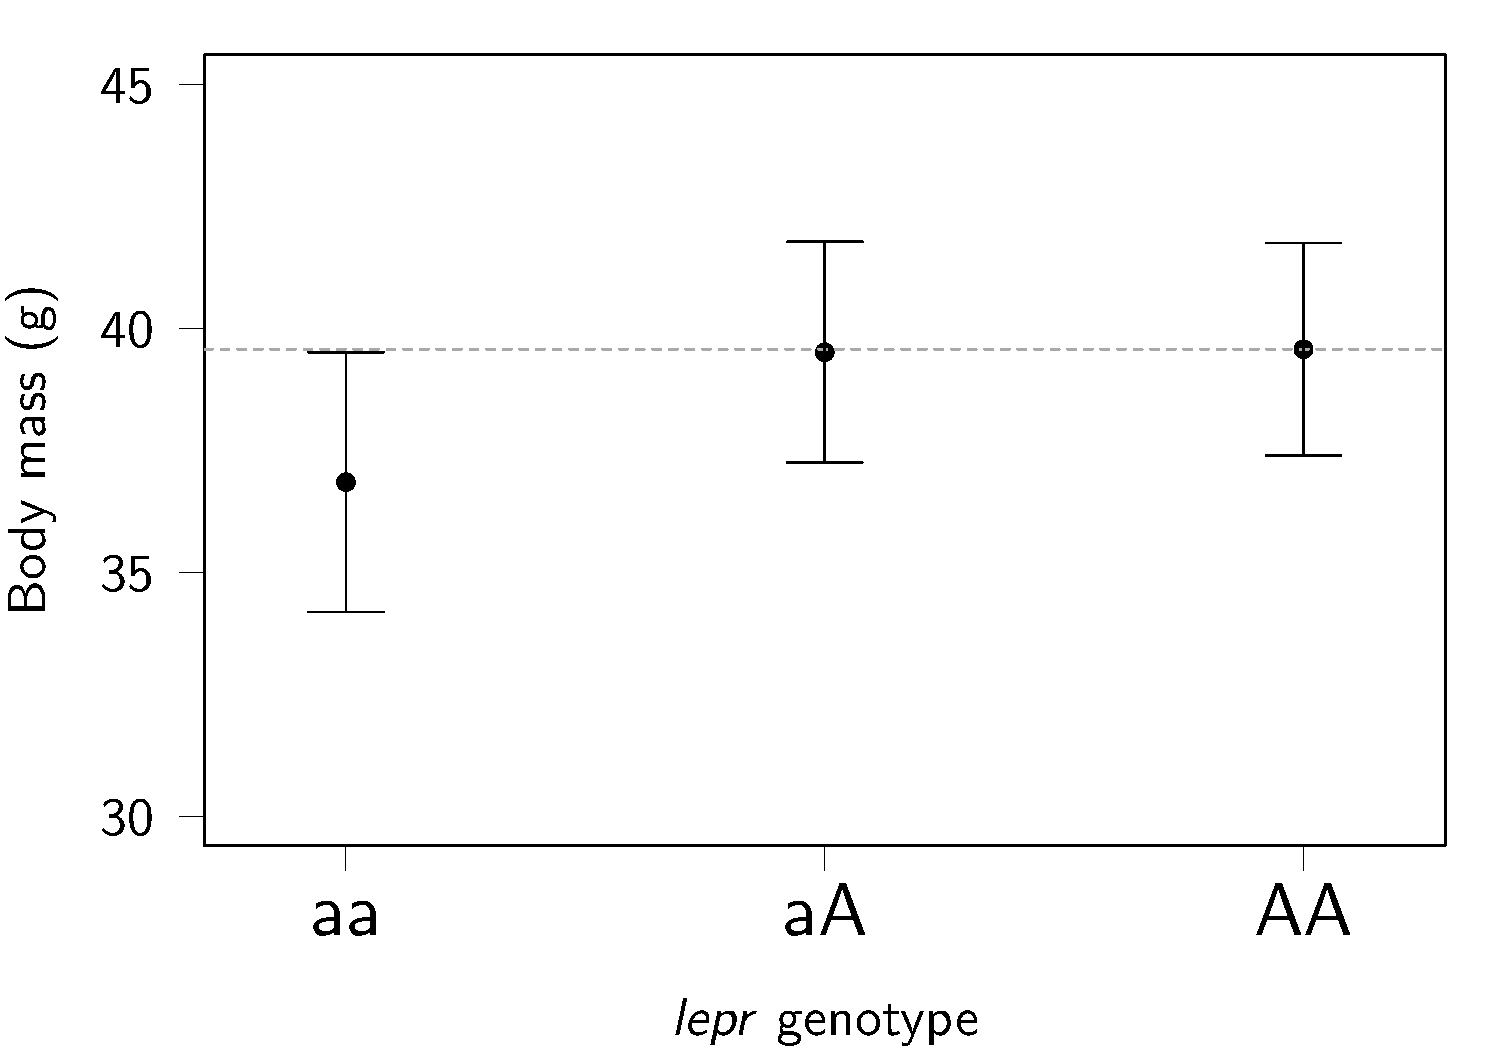
\includegraphics[width=0.5\textwidth]{FiguresGeneral/PhenoEffect-1}
	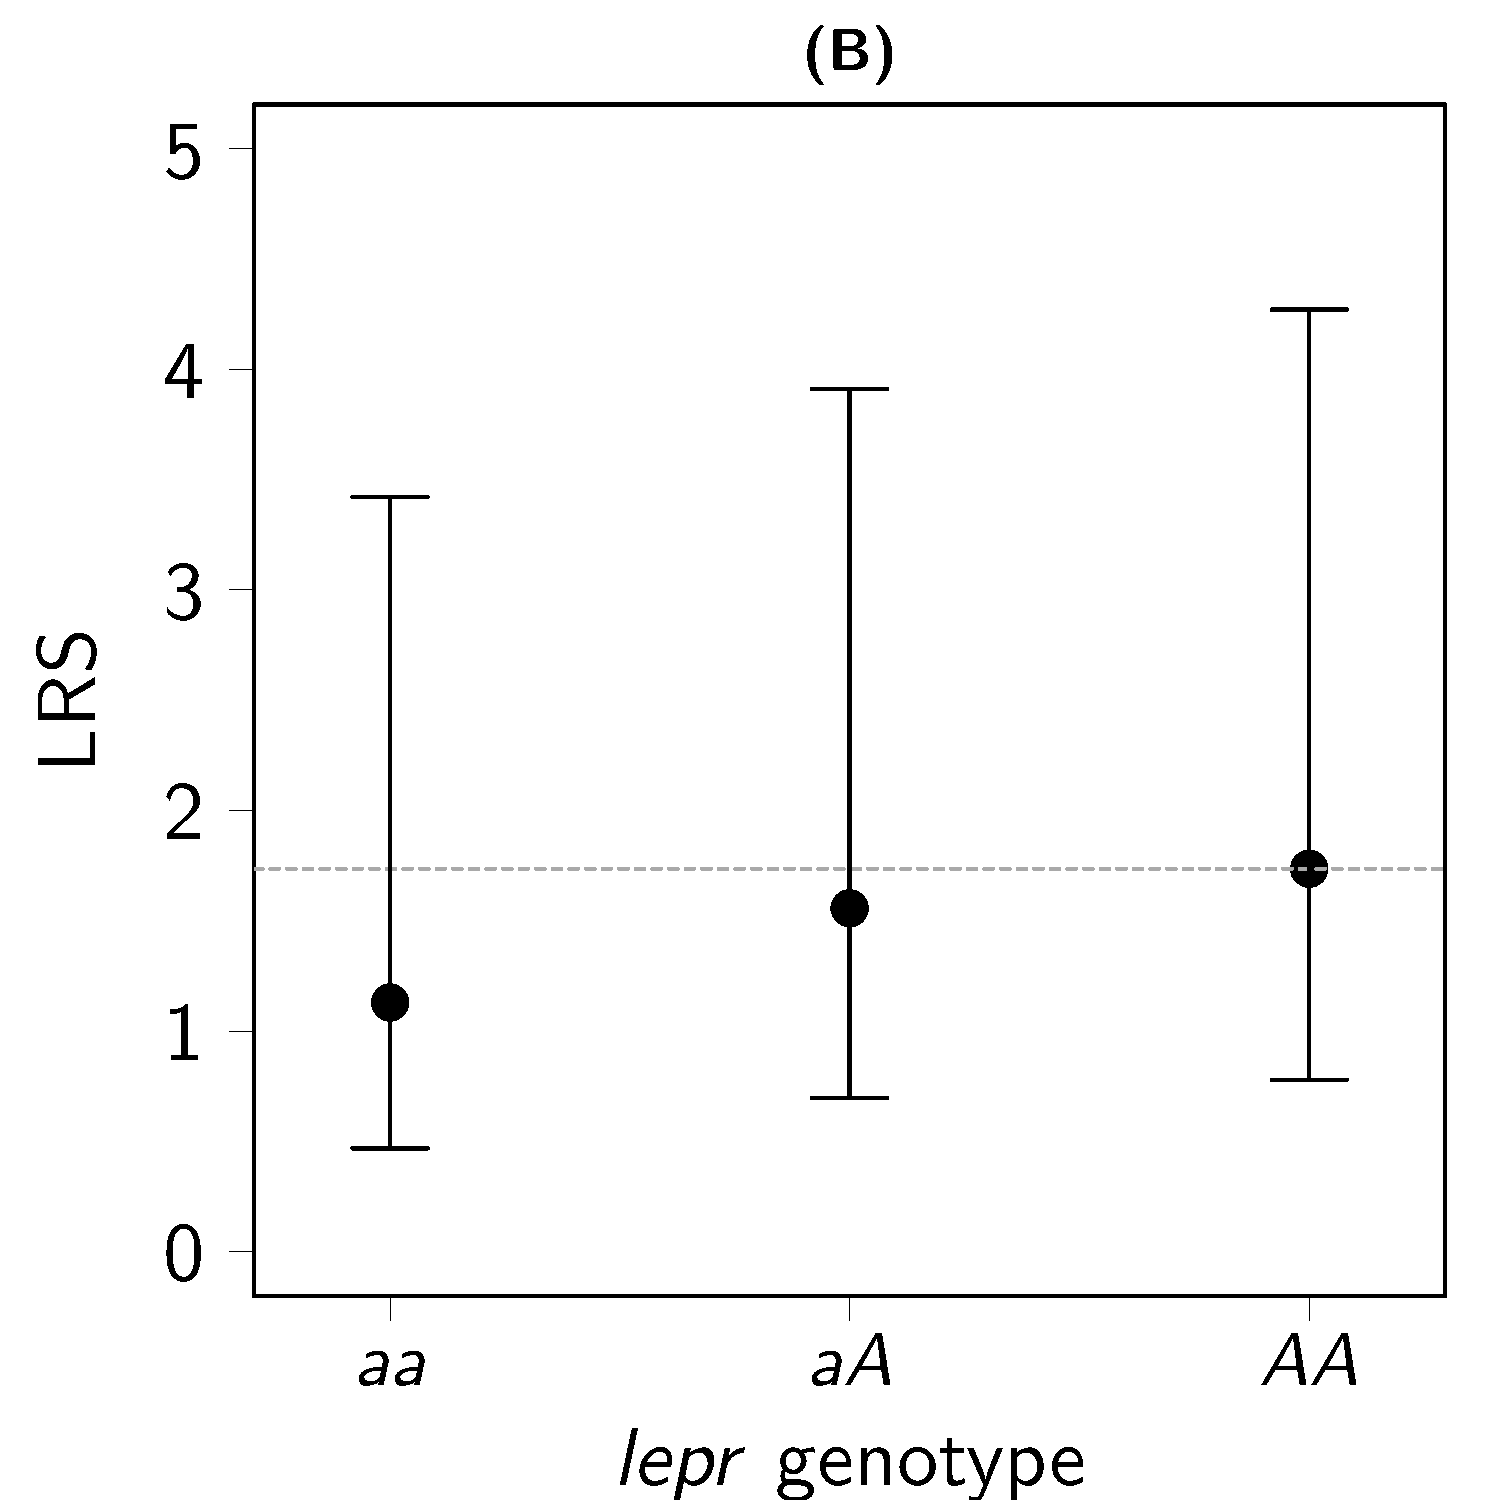
\includegraphics[width=0.5\textwidth]{FiguresGeneral/FitnessEffect-1}
	\caption{Body mass and lifetime reproductive success (LRS) as a function of \emph{lepr} genotypes. 
	(\textbf{A}) Expected body mass of snow voles bearing the three \emph{lepr} genotypes. The expectations and 95\% confidence intervals were predicted from a linear mixed model fitted to the 2311 mass measurement of 532 snow voles. The model accounted for sex, age, date of capture and their two-ways interactions, as well as year of capture and multiple measurements of the same individual.
	(\textbf{B}) Expected LRS of snow voles bearing the three \emph{lepr} genotypes. The expectations and 95\% confidence intervals were predicted from a Poisson generalized linear mixed model fitted to the LRS of 611 snow voles. The model accounted for inbreeding coefficient, year of birth and over-dispersion (using an observation-level random effect). For both panels, the dashed horizontal line projects the expected value of genotype \emph{AA} to ease comparison with \emph{Aa} and \emph{aa}.}
	\label{fig:leprpheno}
\end{figure}

Knowing the effect of the three genotypes and the allele frequencies one can compute analytically the additive genetic variances associated with a bi-allelic locus \parencite[][p77]{Fisher1941average,Lynch1998}. Thus, the additive genetic variances associated with \emph{lepr} are $0.052$  for body mass and $0.006$ for LRS. For both traits, \emph{lepr} explains about 1\% of the additive genetic variation as estimated from an animal model. This is a relatively large proportion for a single locus given that quantitative traits loci typically explain a fraction of a percent to a few percents of additive genetic variance (V$_\text{A}$), when they have a large enough sample size to mitigate Beavis effect \parencite{Flint2009,Jensen2014}.  Still, 1\% of V$_\text{A}$ is not sufficient to infer the evolutionary potential of the trait. Finally, genotyping many more markers, for instance using high-throughput sequencing \parencite{Goodwin2016}, is unlikely to improve this situation in the snow vole population. Generally, very large sample sizes and high-quality genomic resources are necessary to explain a biologically proportion of genetic variances \parencite{Bloom2013, Jensen2014}. For instance 3,925 individuals and 294,831 markers were necessary to explain 45\% of the genetic variation in human height \parencite{Yang2010}. 

%Could we not use high-throughput sequencing techniques to explain a larger proportion of genetic variation, and at the same time identify the genes associated with phenoytpic variation and selection? 
%In theory we could, but in practice this avenue is still a rather laborious and expensive one \parencite{Goodwin2016}. The outcome is also uncertain: 
%The first objective, estimating genetic variances often requires huge sample sizes and number of markers and in general only a small fraction of V$_\text{A}$ is recovered \parencite{Bloom2013}. For instance, even in the most abundant and best known model organism, humans (\textit{Homo sapiens}, Linnaeus 1758), 
%sample sizes of over XXX were necessary to explain 
%XX\% of variation in body mass. 
%Such progresses were accomplished by increasing sample sizes by several order of magnitude and developing Neither can be achieved in small populations of non-model organisms.

%The second objective, identifying the genetic mechanisms of variation and selection, in small populations the number of genetic loci that can be identified with statistical significance can be limited by the problem of multiple comparisons, although solutions are emerging. Moreover, the genotype/phenotype map can hardly be understood from a fully bottom-up approach because of pervasive interactions among genes and with their environment \parencite{Pigliucci2009}. 

To conclude, bottom-up approaches can better unravel the molecular mechanisms underlying phenotypes, but they are not effective at estimating the genetic parameters of phenotypes. On the other hand, quantitative genetics lump all the effects of individual genes and their interactions into only a few parameters, non-informative about the underlying genetic architecture \parencite{Mackay2001,Nietlisbach2015,Huang041434}.  This summarized estimation provides simple and direct measures of genetic parameters. Quantitative genetics work directly on the phenotype which is the target of selection, and the source of ecological interactions. They therefore provide simple measures of genetic parameters that can directly be interpreted within the ecology of organisms.
This thesis is concerned with the genetics and evolution at the level of organisms, in relation to their environment, and accordingly, most of my work relies on quantitative genetics.

%The uncertainty in the estimation of the effect of \emph{lepr} on mass translates into a p-value of $0.01$. Using the widespread arbitrary threshold of $0.05$, If other genetic loci were analysed, using quantitative trait loci mapping or genome wide association


%%%%%%%%%%%%%%%%%%%%%%%%%%%%%%%%%%%%%%%%%%%
\section{This thesis}

\subsection{Objectives}




\subsection{Snow voles in Churwalden}

% Species
The snow vole (\textit{Chionomys nivalis}, Martins 1842) is a medium-sized rodent, its adult body size ranges from 10 to 14 cm, without the tail (5 to 7.5 cm long). Contrary to a widespread intuition, snow voles are not white (Fig. \ref{fig:juvvole}). The fur colour of the upper-parts varies from light to dark taupe grey, sometimes tinted with brown or dark red. This misconception highlights that the species could favourably renamed \emph{rock vole}: it is a rock, rather than a snow, specialist \parencite{Luque-larena2002} and might be associated with high elevations only because rocky areas are more widespread there. It is sparsely distributed across southern Europe and Asia Minor, from sea level up to 4000 m of elevation \parencite{Janeau1997}.
\begin{figure}[ht]
	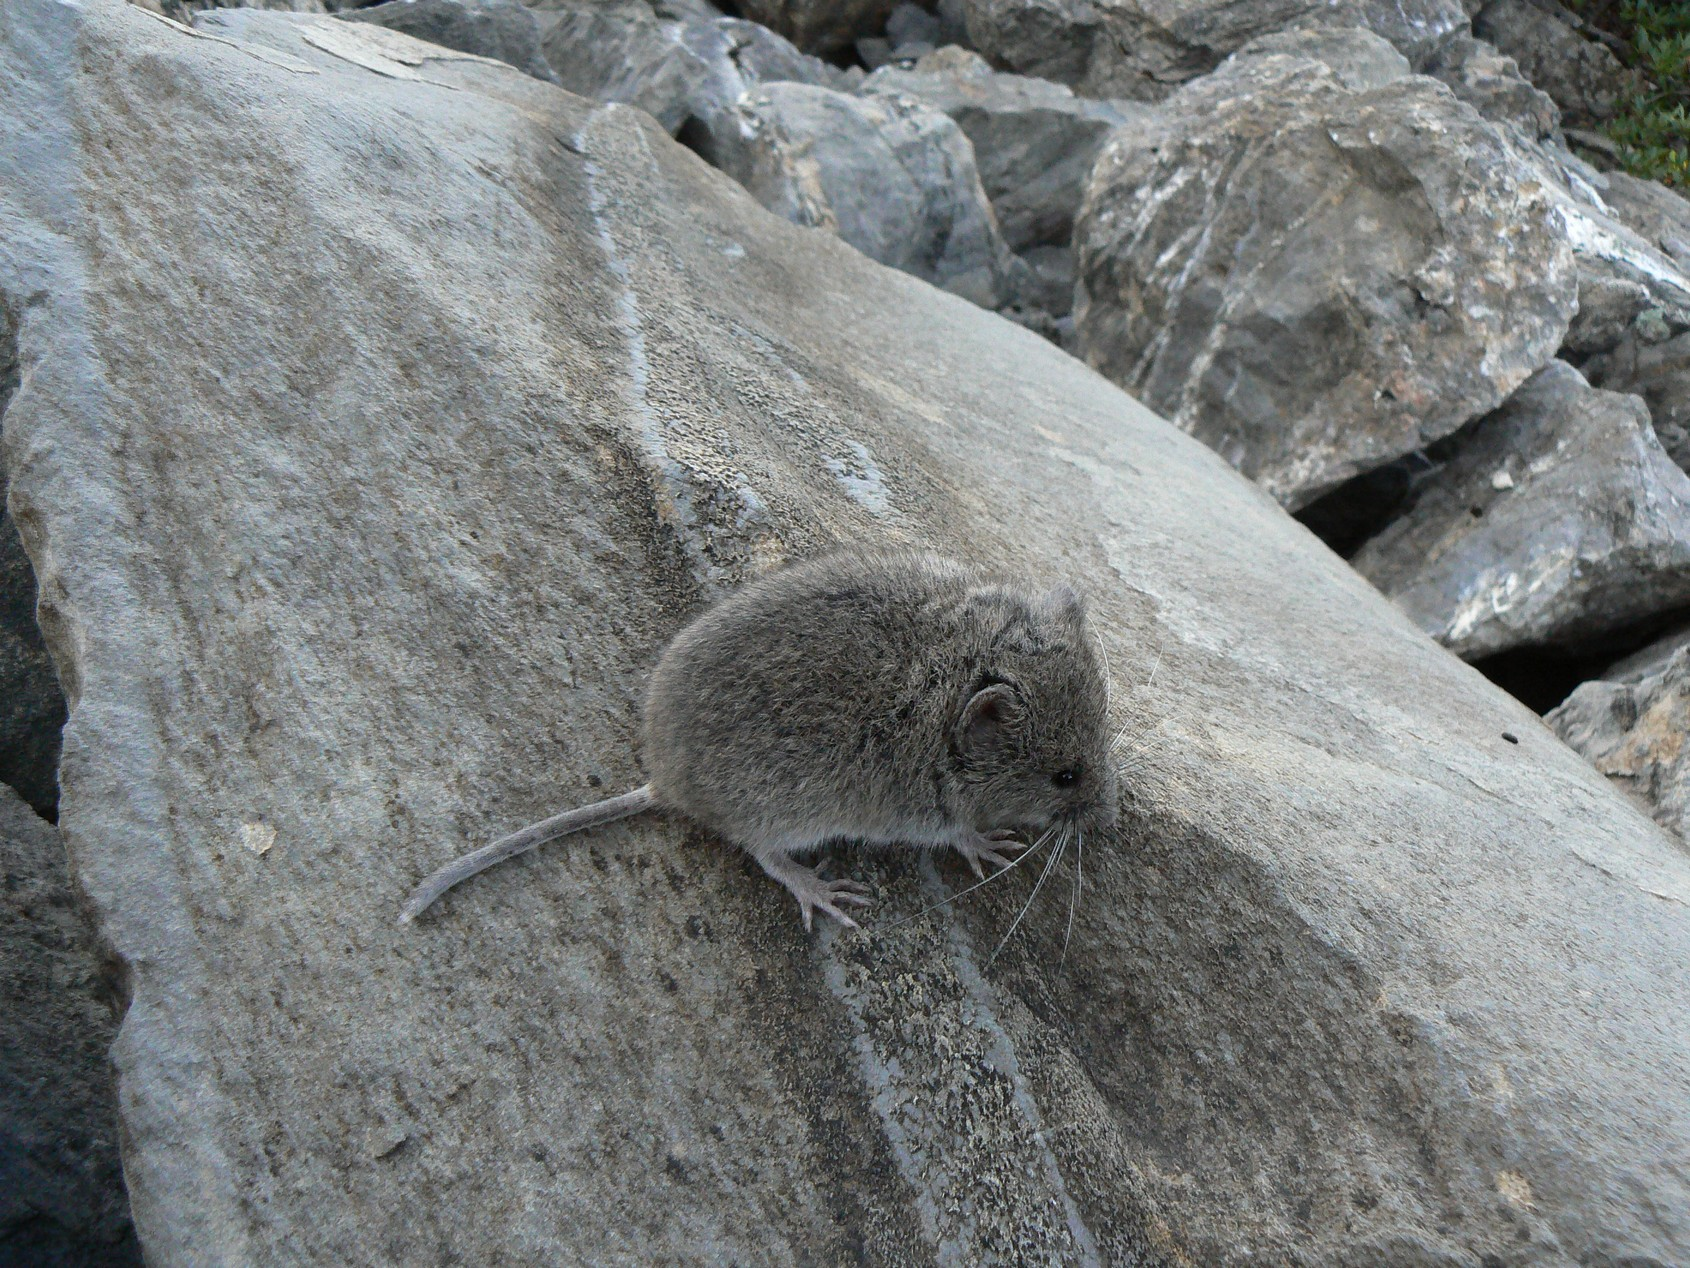
\includegraphics[width=0.49\textwidth]{FiguresGeneral/juvvole.JPG}
	\hspace{0.02\textwidth}
	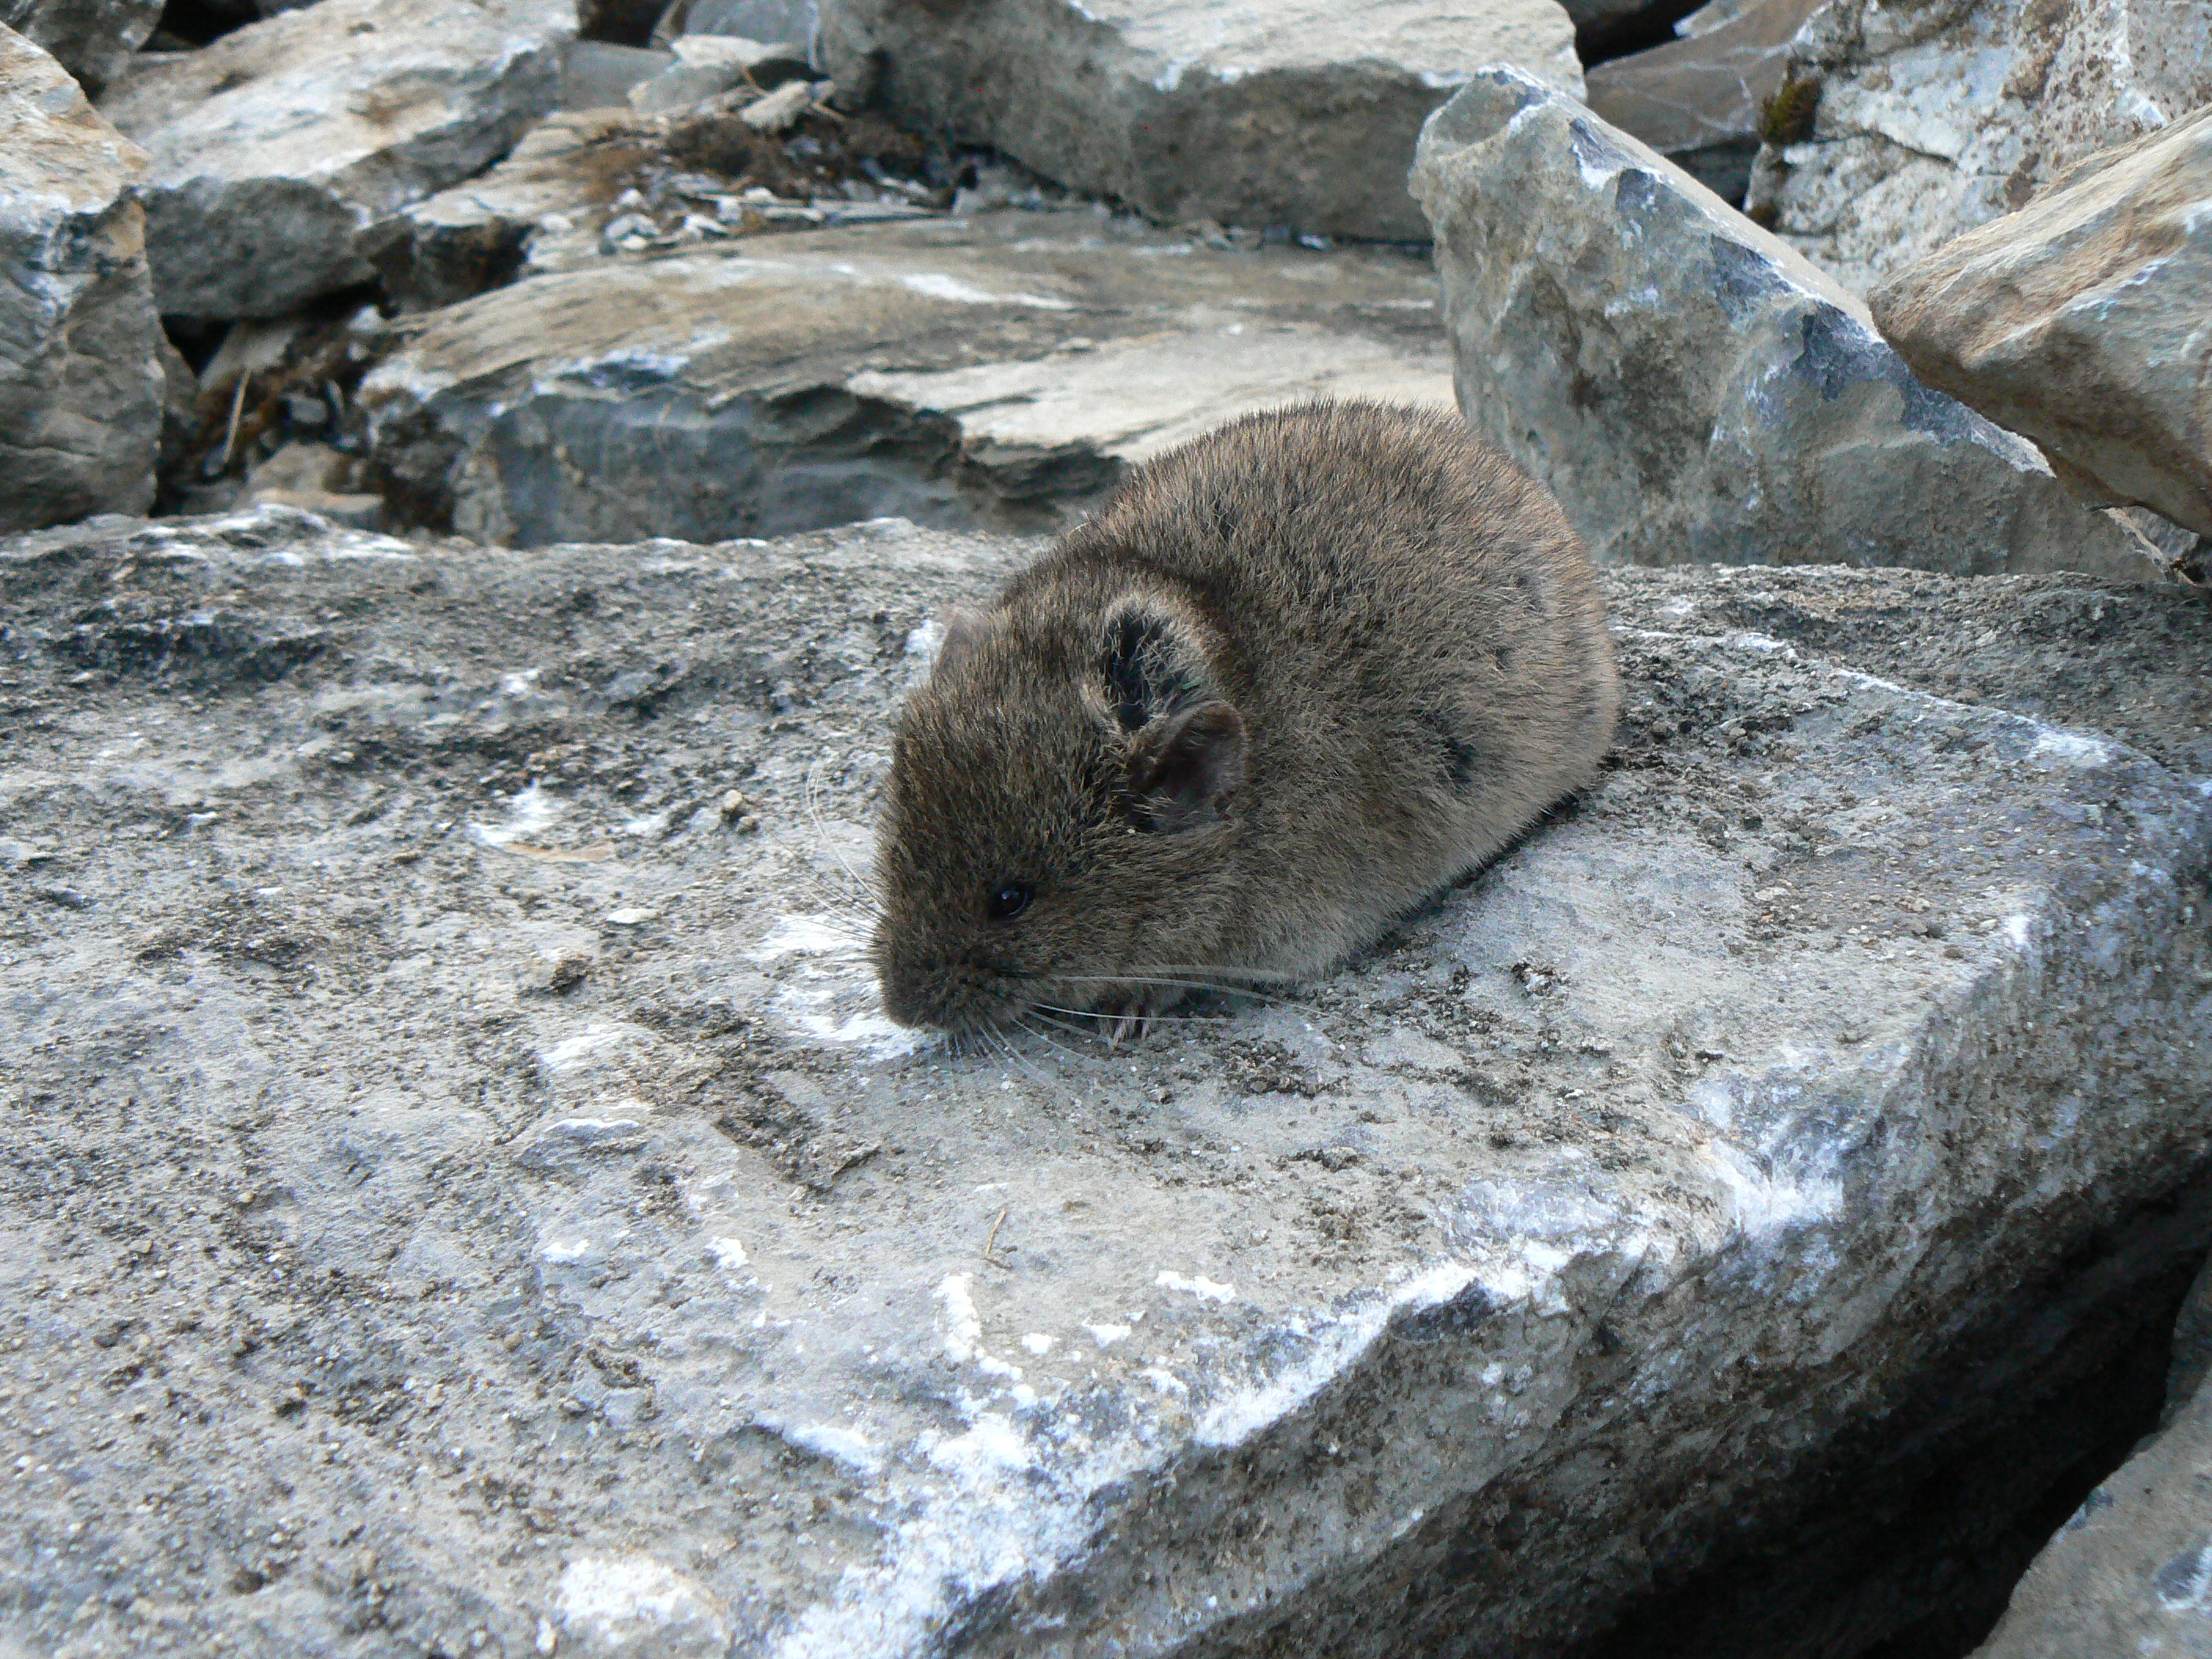
\includegraphics[width=0.49\textwidth]{FiguresGeneral/advole.JPG}
	\caption{Juvenile (left picture) and adult (right picture) snow voles in their habitat in Churwalden, Switzerland. Juveniles always lack the brown hue generally found in adults. Neither adults nor juveniles are white.}
	\label{fig:juvvole}
\end{figure}

Snow voles excavate burrows under the rocks, but can also use natural clefts between rocks sometimes carrying small stones to build walls \parencite{Niederer2008}. A burrow consists of tunnels connecting chambers, one for the nest and multiple ones to stock dry plants \parencite{Janeau1997}. The species is not known to hibernate. 
Adult females actively defend small territories against non-relatives and tend to form matrilineal clusters of territories, whereas adult males wander, and fight, across large overlapping home-ranges \parencite{Luque-larena2004, Garcia-Navas2016}. The matting system is promiscuous and a same litter can be sired by multiple males. Females normally produce 1 to 4 litters of 1 to 5 pups between May and September. Juveniles generally do not reproduce in their first civil year. 
Although they can eat flour worms in the lab, there is no evidence that snow voles are not strictly herbivorous in the wild \parencite{Janeau1997}. In the Swiss Alps, snow voles suffer predation from red foxes, stoats, various owls and corvids, and parasitism from flees, lices and ticks \parencite{Janeau1997, Martinoli2001}.

% Population, characteristics
The study area is located by the Churer Joch, Churwalden, in the Swiss canton Graub\"unden (coordinates $46^{\circ}$48' N, $9^{\circ}$34' E), and covers about 5 ha between 1980 m and 2100 m above sea level. It consist of a west-exposed scree interspersed with small coniferous trees and with patches of alpine meadow. The study area is demarcated by extensive meadows to the south and to the north, by a coniferous forest to the west and by cliff to the east. Another scree, called Wolfgruoben, offers about 1 ha of favourable habitat, starting 300 m north-east to the monitored area. Wolfgruoben was trapped in 2008 and 2013. The snow vole density was rather low, with on average five captures per night of trapping, versus 18 on the main study area. More habitat favourable to snow voles can be found 2 Km to the south. The study population is moderately isolated and receives 5 to 10 immigrants per year \parencite{Garcia-Navas2016}. 

% Monitoring and history
The monitoring of this snow vole population was initiated in 2006 by Dr. Peter W. Wandeler. Dr. Erik Postma took the monitoring over in 2012, but the protocol has remained practically unchanged. This thesis contains data collected up to the year 2015.
\begin{figure}[ht]
	\begin{tikzpicture}
		\node (pic) at (0,0) {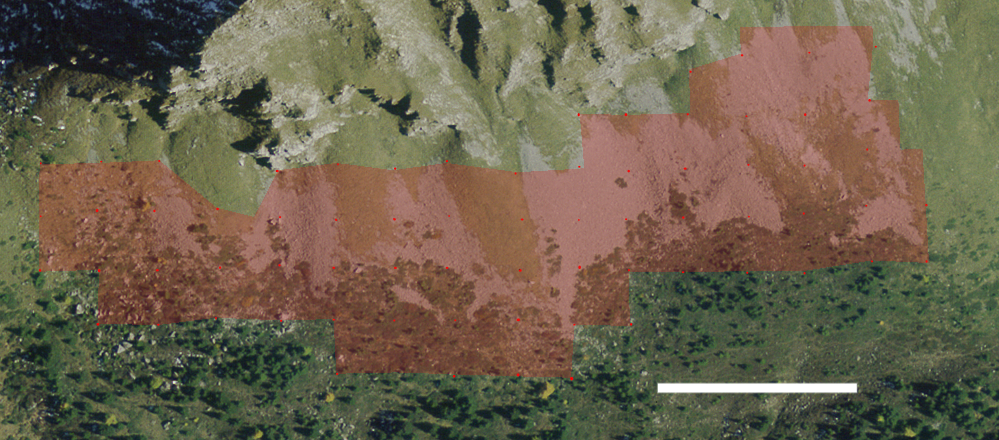
\includegraphics[width=1\textwidth]{FiguresGeneral/fieldposts2.PNG}};
		\draw[<-, ultra thick, color=white,>=stealth] (6.5,-2.5)--(7.5,-2.65);
		\node (n) at (6.3,-2.4) {\color{white}{N}};
		\draw[ultra thick, color=black] (2.52,-2.59)--(2.52,-2.75)--(5.68,-2.75)--(5.68,-2.59);
		\node (m) at (4.1,-3) {\color{white}{100 m}};
		%\draw[ultra thick, color=black] (2.52,-2.75)--(2.52,-2.65);
		%\draw[ultra thick, color=black] (5.68,-2.75)--(5.68,-2.65);
	\end{tikzpicture}
	\caption{Orthophoto of the study site, from 2008. The red shading indicates the approximate area where traps are set.}
	\label{fig:fieldarea}
\end{figure}
Every year from 2006 to 2016, snow voles were life-trapped multiple times between late May and early October. Traps were set during the day, opened around sunset and checked the next morning. 
For every snow vole capture \footnote{Other species (bank voles, pine voles, wood mice, stoats, black salamanders, slugs\dots) were released without taking measurements.}, we recorded sex, age, body mass, body length, tail length, date, location and signs of reproductive activity (pregnancy, lactation, swollen scrotum). 
In addition, all newly-captured snow voles were individually marked and genotyped for 18 microsatellites \cite{Wandeler2008}. Based on the autosomal microsatellite genotypes, we reconstruct the pedigree of the population. This pedigree is the raw material for most of the work carried out during this thesis. In particular, the pedigree is used to define reproductive success, as well as to estimate the relatedness between all pairs of individuals. These two statistics are essential to estimate selection, fitness and genetic variation. 


\subsection{Thesis outline}

\printbibliography[heading=subbibliography]

